
% ----------------------------------------------------------------------
\section{Results}
\label{sec:results}
% ----------------------------------------------------------------------

Using climate forcing from WordClim data and the NCEP/NCAR, ERA-Iterim, CFSR and NARR reanalyses described in section~\ref{sec:climate} and the ice sheet model described in section~\ref{sec:model}, we run simulations of glacial inception and growth of the Cordilleran ice sheet using different temperature offsets.

\begin{figure}[t]
	\vspace*{2mm}
	\begin{center}
		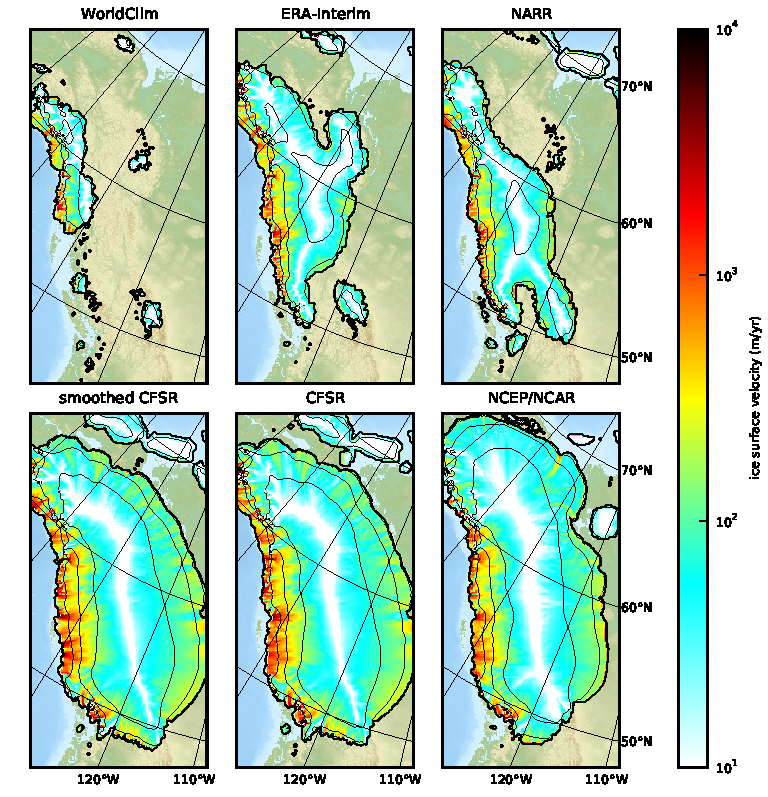
\includegraphics[width=13cm]{cordillera-climate-cool06}
	\end{center}
	\todo[inline]{Change panel order to match climate section}
	\caption{Ice surface topography (black contours every 1000\,m) and velocity (\unit{m\,yr^{-1}}) after 10\,kyr under a climate 6\degC colder than present for each climate forcing.}
	\label{fig:cool06}
\end{figure}

Figure~\ref{fig:cool06} shows the effect of a 6\degC temperature offset on the six different climate forcings. It apperas that the magnitude of glaciation differs highly between forcing datasets. NCEP/NCAR and CFSR forcings produce large ice sheets covering parts of Yukon and Alaska which are thought to have remained unglaciated for at least several glacial cycles. \needref The smoothing of CFSR precipitation has limited effect on the resulting ice sheet geometry. The WorldClim forcing results to a glaciation mode limited to major mountain ranges, whereas ERA-Interim and NARR produce medium-sized ice sheets with a difference in shape.

\begin{figure}[t]
	\vspace*{2mm}
	\begin{center}
		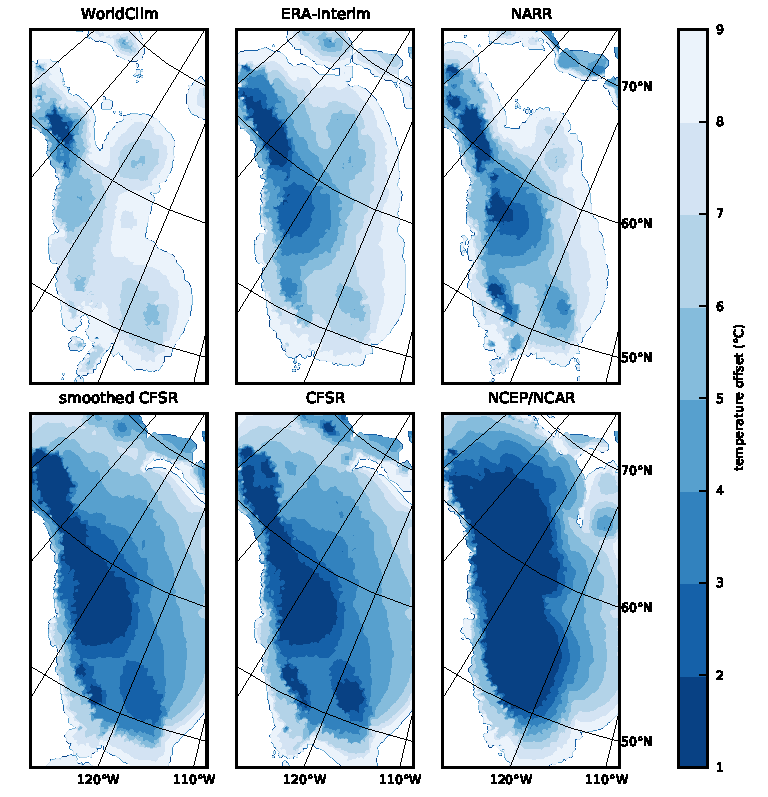
\includegraphics[width=13cm]{cordillera-climate-extent}
	\end{center}
	\todo[inline]{Change panel order to match climate section}
	\qiong[inline]{Move ticks on the colorbar. The 1 is confusing.}
	\caption{Extent of ice cover after 10\,kyr as a function of applied temperature offsets for each climate forcing.}
	\label{fig:extent}
\end{figure}

As we aim to model an ice sheet approaching LGM size, yet do not know how cold was the climate shaping it, we apply temperature offsets ranging from 2 to 9\degC for each climate forcing. Figure~\ref{fig:extent} shows the extent of ice cover at the end of each of theses 40~simulations, grouped by climate forcing. Again it is visible that different forcings lead to very different final ice cover, generally. Notably, for the lowest temperature offset of 2\degC, NCAR and CFSR simulatinos lead to a significant ice-sheet, whereas WorldClim, NARR and ERAI produce mountain ice caps, not more extensive than present for WorldClim. It should be noted that several of the NCAR and CFSR simulations producve oversised ice-sheets whose extent is primirily bounded by the model domain boundary conditions rather than any physical process. Where different climate forcings lead to similar ice sheet sizes, differences in pattern can be noted. For instance ERAI ice seets appear more northernly-centered than NARR ice sheets.

\begin{figure}[t]
	\vspace*{2mm}
	\begin{center}
		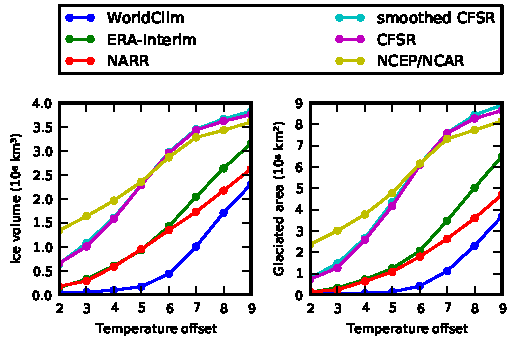
\includegraphics[width=9cm]{cordillera-climate-ivolarea}
	\end{center}
	\todo[inline]{Use black-and-white-proof markers}
	\todo[inline]{Highlight the ``best'' runs.}
	\caption{Total ice volume and glaciated area after 10\,kyr as a function of temperature offset and climate forcing.}
	\label{fig:ivolarea}
\end{figure}

Figure~\ref{fig:ivolarea} shows the final ice volume and glaciated area at the end of each of the 48~simulations. Differences in ice sheet size can be quantified. ERAI and NARR lead to similar ice volumes and glaciated areas, yet patterns are different as shown by Figure~\ref{fig:extent}.

\begin{figure}[t]
	\vspace*{2mm}
	\begin{center}
		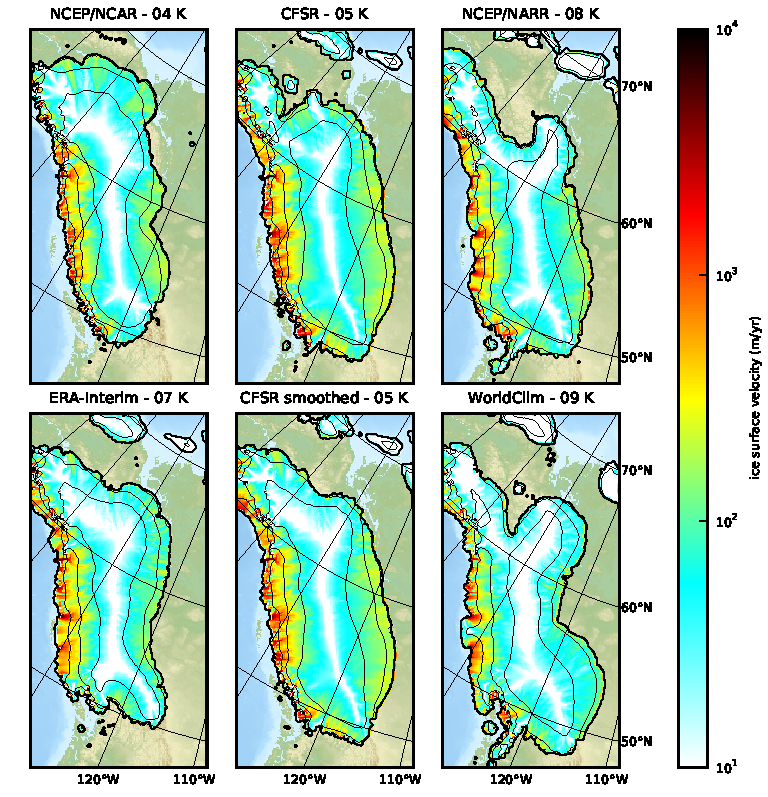
\includegraphics[width=13cm]{cordillera-climate-best}
	\end{center}
	\todo[inline]{Change panel order to match climate section}
	\caption{Ice surface topography (black contours every 1000\,m) and velocity (\unit{m\,yr^{-1}}) after 10\,kyr using temperature offsets that lead to similar areas of ice cover for each climate forcing.}
	\label{fig:best}
\end{figure}

To be able to compare runs of similar magnitudes, and as we consider temperature offset as an unknown in this study, we select for each climate forcing the simulation that lead to most realistic results in terms of glaciated area. This was done by using the LGM extent countour from \needref shown in Figure~\ref{fig:locmap}, which covers an area of XXX \todo{do the maths}. These so called ``best'' runs are presented in Figure~\ref{fig:best} along with the temperature offset values associated.

